An array is a finite, ordered list of similar objects. These objects can be arrays themselves. An array nested inside another array is called subarray. All subarrays inside an array have the same structure. Accordingly, an array can be seen as ordered, finite, nested lists of objects. The objects are accessed by their position in the list called index. The index ranges from $0$ to size$-1$. The size is the number of objects inside the array. Accessing an object is denoted by square brackets. For example, the object $a[2]$ at index $2$ in the array $a = [a,b,c,d]$ is $c$.\autocites{Black.2016}{Garcia.2005}
Another way to denote accessing an object of a multidimensional array is to separate the indices of different dimensions by a comma. Given a multidimensional array $a$, an object at the indices $i_1, i_2, \dots, i_n$ is denoted $a[i_1, i_2, \dots, i_n]$
with $i_d$ being the index in the $d$th dimension, $n \in [1;D]$, and $D$ being the number of dimensions of $a$. For example, given the array~$a$ of Table \ref{tab:array}, the object $a[0,0] = a[0][0]$ is $[1,2,3]$. \autocite{Castro.2010}
\par
An array can be described by its dimensionality and shape.
The dimensionality or number of dimensions is the nesting depth of an array.
The shape of an array is denoted by its size $\times$ the shape of its subarrays. If the array contains no subarrays its shape is denoted by its size. Thus, the product of all sizes in the shape is the total number of objects contained in an array.\autocites{Black.2016}{Garcia.2005} This is illustrated in Table \ref{tab:array}.
\begin{xltabular}{\textwidth}{cccc}\toprule
	\caption{Array} \label{tab:array}\\
	\textbf{Array} & \textbf{Contents} & \textbf{Shape} & \textbf{Dimensionality} \\\midrule \endhead
	$a$ & $
	\begin{bmatrix}
	\begin{bmatrix}
	\begin{bmatrix}
	1 & 2 & 3
	\end{bmatrix}\\
	\begin{bmatrix}
	4 & 5 & 6
	\end{bmatrix}\\
	\begin{bmatrix}
	7 & 8 & 9
	\end{bmatrix}	
	\end{bmatrix} &
	\begin{bmatrix}
	\begin{bmatrix}
	1 & 2 & 3
	\end{bmatrix}\\
	\begin{bmatrix}
	4 & 5 & 6
	\end{bmatrix}\\
	\begin{bmatrix}
	7 & 8 & 9
	\end{bmatrix}	
	\end{bmatrix} &
	\begin{bmatrix}
	\begin{bmatrix}
	1 & 2 & 3
	\end{bmatrix}\\
	\begin{bmatrix}
	4 & 5 & 6
	\end{bmatrix}\\
	\begin{bmatrix}
	7 & 8 & 9
	\end{bmatrix}	
	\end{bmatrix}
	\end{bmatrix}
	$ & $3 \times 3 \times 3$ & $3$\\\midrule
	$a[0]$ & $
	\begin{bmatrix}
	\begin{bmatrix}
	1 & 2 & 3
	\end{bmatrix}\\
	\begin{bmatrix}
	4 & 5 & 6
	\end{bmatrix}\\
	\begin{bmatrix}
	7 & 8 & 9
	\end{bmatrix}	
	\end{bmatrix}
	$ & $3 \times 3$ & $2$\\\midrule
	$a[0][0]$ & $
	\begin{bmatrix}
	1 & 2 & 3
	\end{bmatrix}
	$ & $3$ & $1$
	\\\bottomrule
\end{xltabular}


\par
In this paper, an array is used to generalize matrices and vectors for an arbitrary number of dimensions. 
A vector~$\vec{v}$ is seen as a one-dimensional array~$v$ with each scalar $\vec{v}_i$ being the object $v[i]$ with index~$i$.
A matrix $A$ is seen as a two-dimensional array $a$ with each scalar $A_{ij}$ being the object~$a[i][j]$ with row index~$i$ and column index~$j$.
\subsection{Array Visualization}
In the context of a \ac{CNN}, sometimes arrays are visualized. \autocites{Singh.2020}{ElAmir.2020}
In this paper, a three-dimensional array with shape $w \times h \times d$ is visualized as a cuboid of width $w$, height $h$, and depth $d$.
A two-dimensional array with shape~$w \times h$ is visualized as a cuboid or rectangle of width~$w$, height~$h$, and depth~$1$.
A one-dimensional array with shape~$w$ is visualized as cuboid or rectangle of width~$w$, height~$1$, and depth~$1$. \autocites{Ertel.2016}{Rawat.2017}{Sabour.2017}{Krizhevsky.2012}{LeCun.2015b}
This is illustrated in Figure \ref{fig:array}.
\begin{figure}[H]
	%\cube{x offset}{y offset}{width}{height}{depth}{color}{fillcolor}

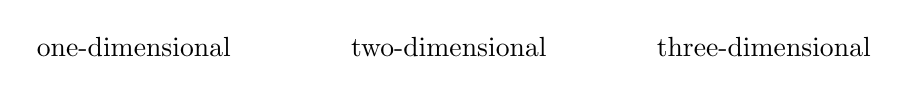
\begin{tikzpicture}[
cell/.style={
	rectangle, 
	rounded corners=2mm, 
	draw,
	very thick,
	align=center,
},
ArrowC1/.style={% Arrows with rounded corners
	rounded corners=.25cm,
	thick,
},
]
\cube{0}{0}{3}{3}{3}{black}{gray}
\cube{-4}{0}{3}{3}{1}{black}{gray}
\cube{-8}{-2}{3}{1}{1}{black}{gray}

\node (3d) at (-1.5,-4,0) {three-dimensional};
\node (2d) at (-5.5,-4,0) {two-dimensional};
\node (1d) at (-9.5,-4,0) {one-dimensional};

\end{tikzpicture}
	\caption{Array Visualization (own figure)}
	\label{fig:array}
\end{figure}
\subsection{Array Slice}
Given an array $a$, an array slice is denoted $a[start:end]$. $a[start:end]$ is defined as $a$ containing only the objects with indices in the range of $start$ to $end-1$. For example, given an array $a=[0,1,2,3,4,5]$, the array slice $a[1:3]$ is $[1,2]$. \autocite{Castro.2010}